%!TEX root = ../thesis.tex

\section{Preliminaries}
\thispagestyle{plain}
\fxinnote{Lead in paragraph}
\fxinnote{define notations and concepts in one go}
\fxinnote{state results at and of this section}

\mypar{Adjacent vertices and chords}
  \fxnote{introduce where this gets relevant}
  We call a vertex \emph{$\pS$-adjacent} when it is adjacent to $\pS$ in the current corner assignment. In the same way we call a chord or $2$-chord \emph{$\pE$-bound}, \emph{$\pW$-bound} or \emph{polebound} when it is adjacent to $\pE$, $\pW$ or any pole,  respectively.

\mypar{Fans}
  We introduce some more concepts to describe the interior of a blue (or red) face. Every interior edge of this face goes from one fence to the other (otherwise its start or end vertex would violate the interior vertex condition).\fxnote{This could be a useful result in the section about cycles and their interiors.} To better understand the structure of such a strip we will describe the edges from $\spl(F)$ to $\mrg(F)$ .

  Let $u_0 , u_1, \ldots u_n$ be the vertices of the upper boundary path of $F$ and $v_0, v_1, \ldots, v_m$ the vertices of the bottom boundary path. That is $u_0=v_0 = \spl(F)$ and $u_n = v_m = \mrg(F)$. Since our graph is a triangulation $u_1v_1$ must be an edge. For the second edge in the face we have two options $u_1v_2$ or $u_2v_1$, otherwise this edge and the previous one would not form a triangle. This principle holds for every subsequent edge, we can either increase the index of the upper boundary path or the index of the bottom boundary path. In other words, this face is a so-called \emph{triangle strip}.

  We call a maximal sequence of at least two edges increasing the index on the bottom boundary path (and thus keeping the index on the upper path fixed) a \emph{Bottom-fan} or simply \emph{B-fan} and a maximal sequence of at least two edges increasing the index on the upper boundary path is called a \emph{Top-fan} or just \emph{T-fan}. \fxnote*{Q What's wrong here?}{The \emph{size} of such a fan is the number of edges contained in the sequence}. By the definition of a fan it has size of at least $2$.
  We use \emph{fans} to refer to both these \emph{types} of fans (i.e. T- and B-fans).
  We call a fan of size $3$ or larger a \emph{large fan} and a fan of size $2$ a \emph{small fan}.

  In a strip we alternately encounter B- and T-fans. Since if we would have two adjacent fans of the same type we would just have a single larger fan of that type.
  In Figure \ref{fig:uni:fans} we see a strip consisting of subsequently a B-fan of size $3$, a T-fan of size 2, a B-fan of size $2$, a T-fan of size $6$, a B-fan of size $3$ and a T-fan of size $3$.

  \begin{figure}[h]
    \centering
    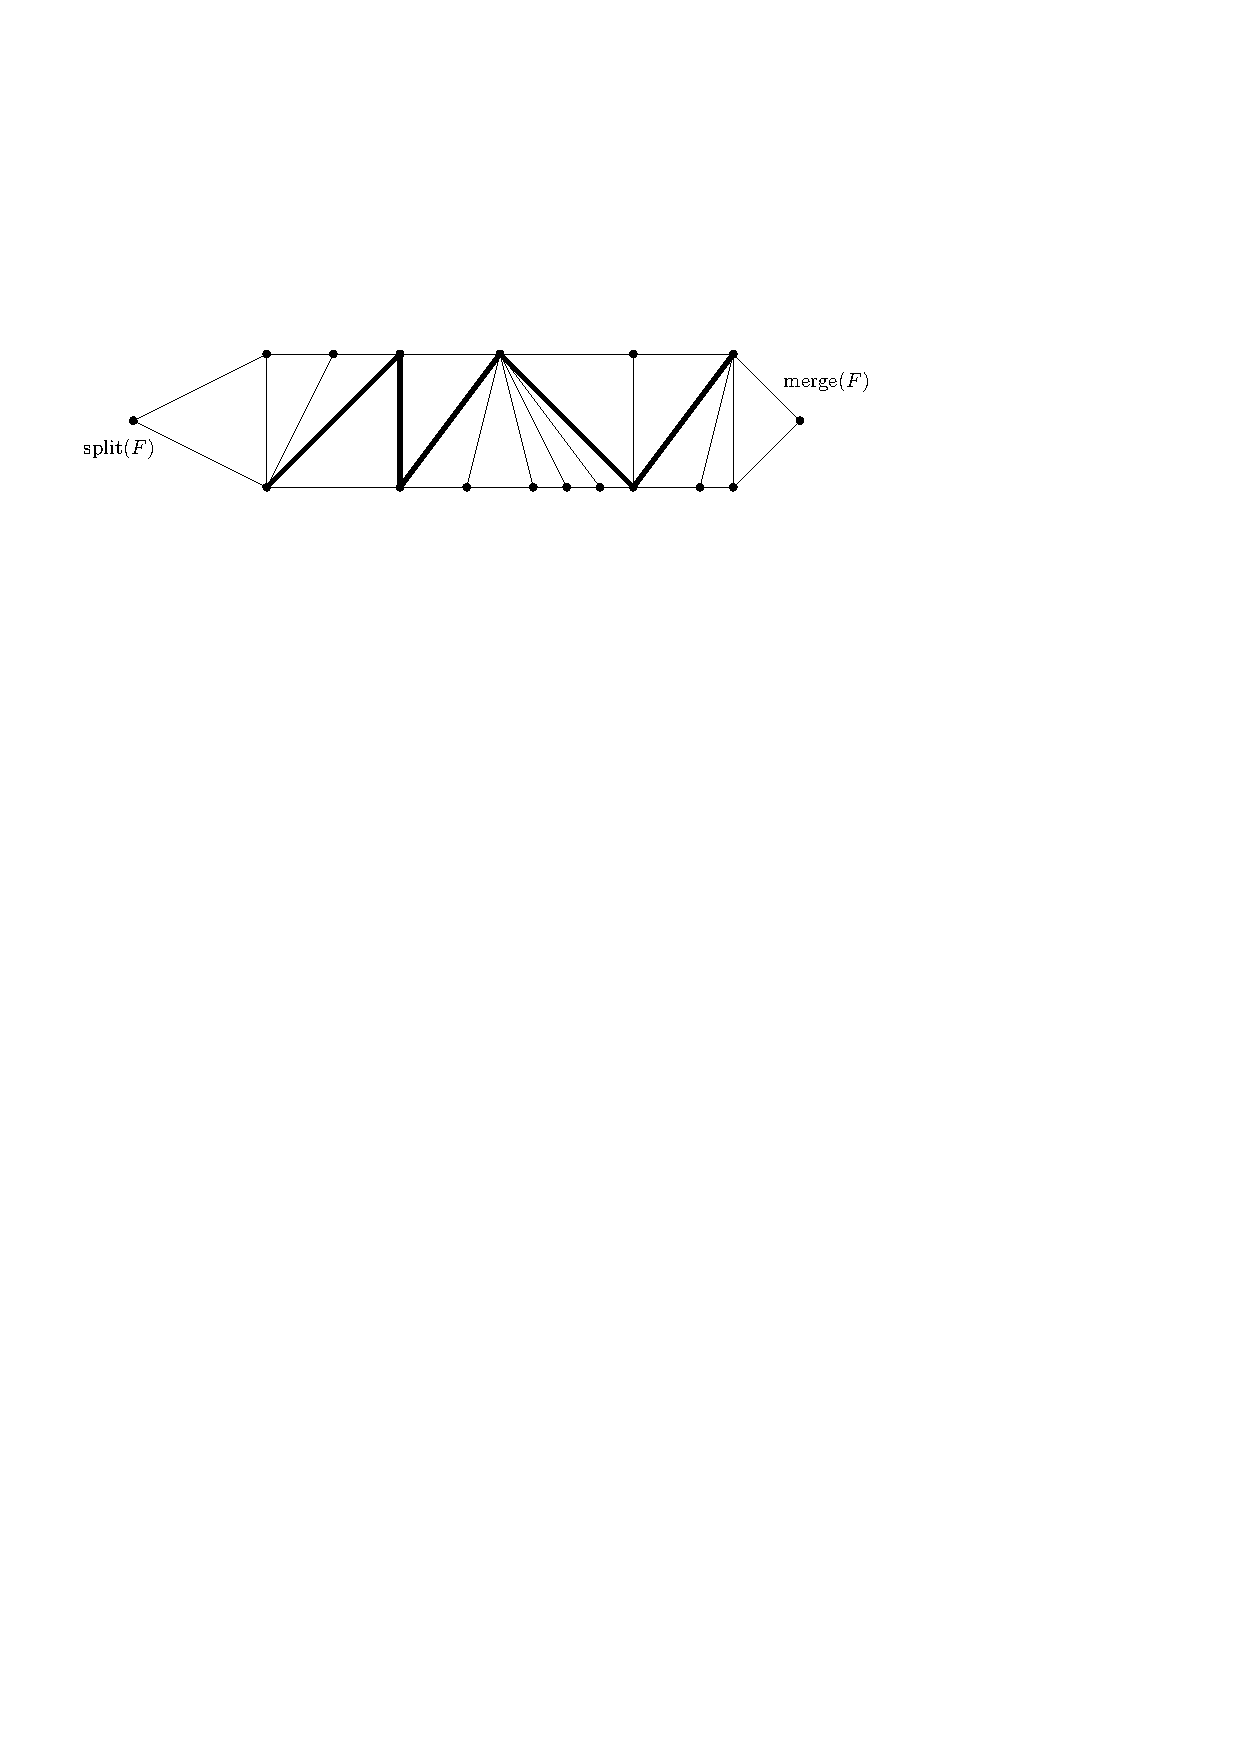
\includegraphics[scale=.9]{rectangularDuals/img/fans}
    \caption{}
    \label{fig:uni:fans}
  \end{figure}


 We introduce some more terminology for fans: \emph{outer edges}, \emph{fan handles} and the \emph{rim} as can be seen in Figure \ref{fig:rect:fanTerms}. The \emph{fan handle} $v$ is the vertex shared by all edges in the fan. Let $F$ be the induced subgraph of vertices adjacent to the edges in the fan. $F$ contains no edges not belonging to the triangle strip since these would lead to separating 3-cycles. The \emph{rim} is the path given by $F\sm{v}$.
 \fxnote{Q is this definition of Rim more clear or still unclear?}
 \fxnote*{Do we use this}{The \emph{outer rim} are the two extreme edges of this path and} the \emph{outer edges} are the edges between the fan handles and the extreme vertices of the \emph{rim}.

 \begin{figure}[h]
   \centering
   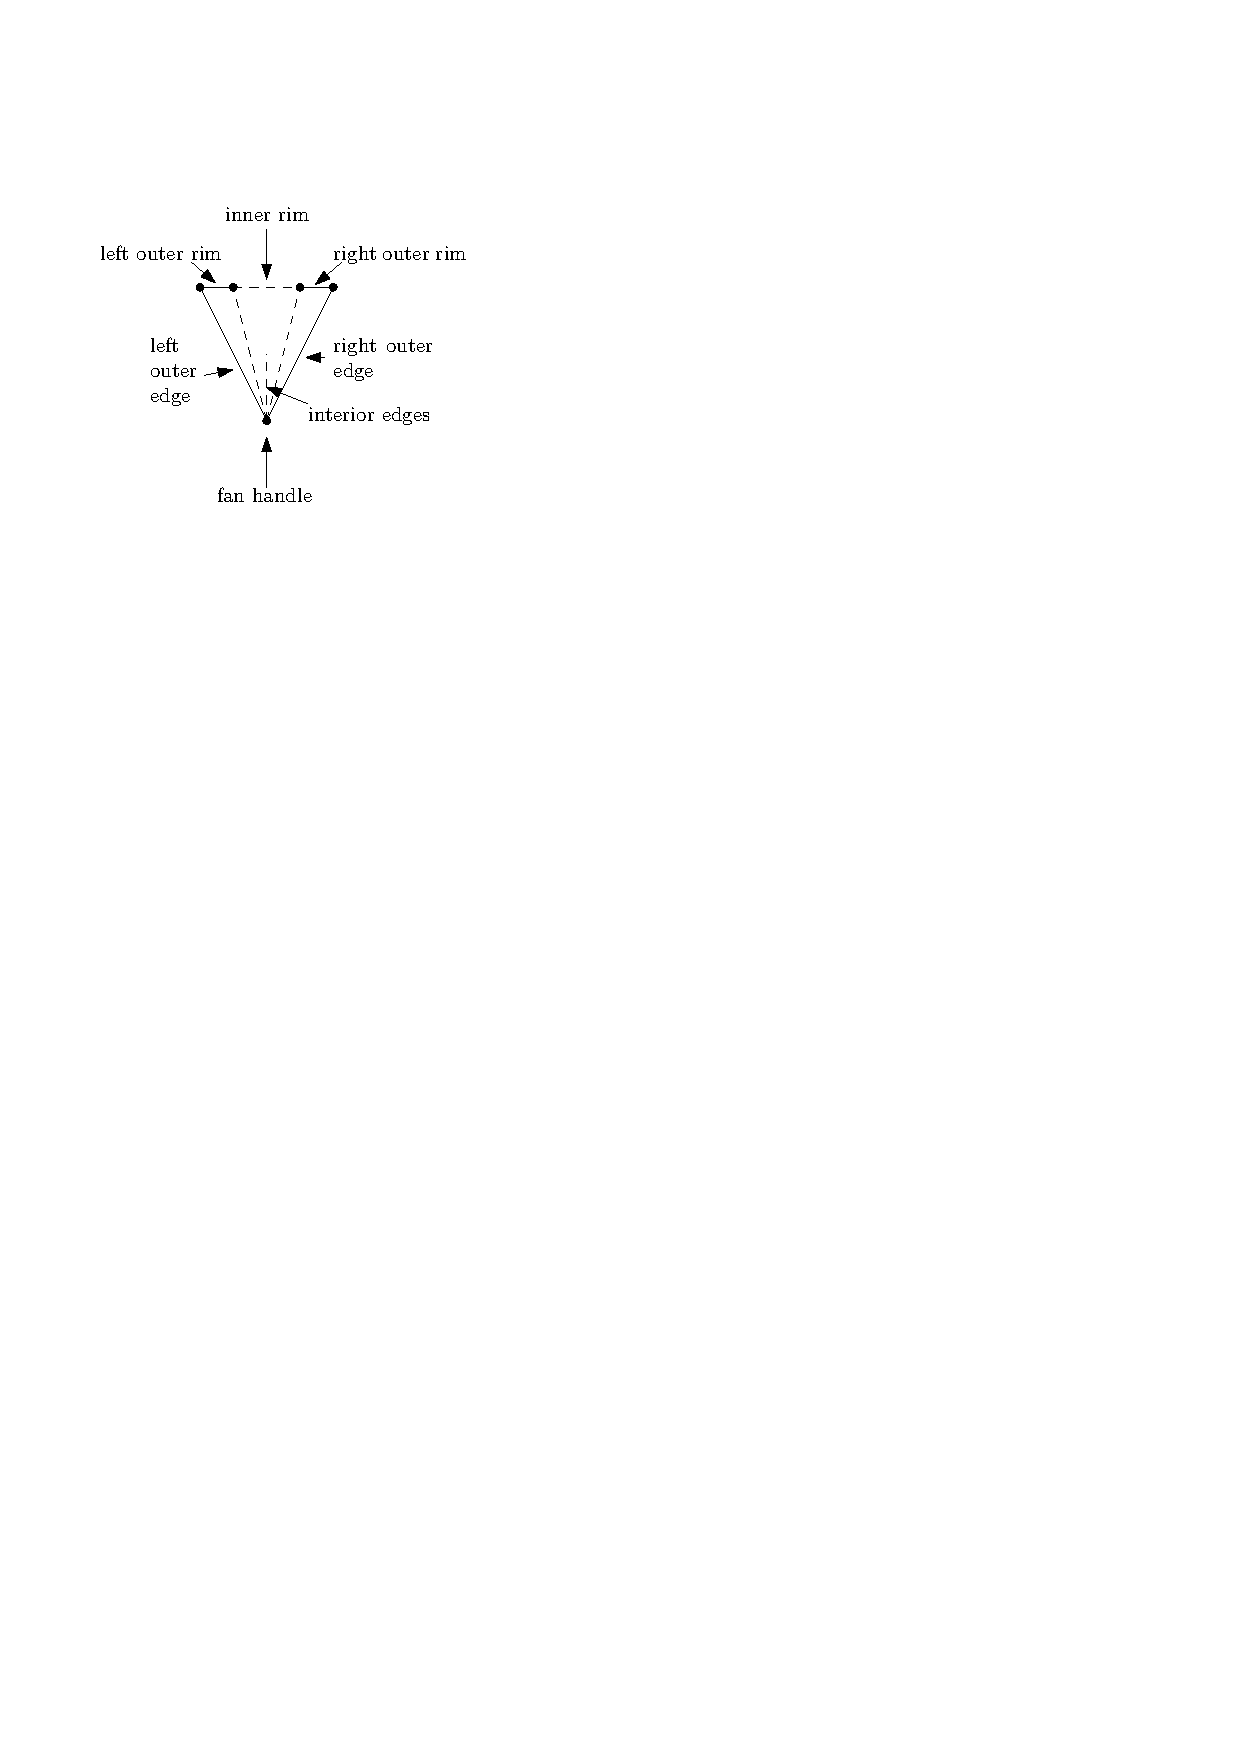
\includegraphics[scale=1]{rectangularDuals/img/fanterms}
   \caption{}
   \label{fig:rect:fanTerms}
 \end{figure}



 \subsection{Different kinds of rectangular layouts}
   A rectangular layout $\L$ can have different properties.
   Recall that $\L$ is area-universal if, no matter the areas we assign to the rectangles of $\L$, some combinatorially equivalent layout $\L'$ has rectangle of the assigned areas.
   Recall also that a \emph{maximal line segments} (or simply \emph{maximal segments}) of $\L$ is a line segment not contained in any other line segment. That is, it can not be extended any further. In this definition a \emph{line segment} (or simply \emph{segment}) of $\L$ is a sequence of consecutive inner boundary segments forming a line.
   A segment is \emph{one-sided} if it is on the boundary of a single rectangle. We call it \emph{$k$-sided} if on one of the sides it is the boundary of at most $k$ rectangles.


   We say a layout \emph{one-sided} if all maximal segments are one-sided.
   Furthermore,  we say it is \emph{vertically one-sided} or \emph{horizontally one-sided} if all vertical or horizontal maximal segments are one-sided, respectively. Finally, a layout is \emph{$k$-sided} if all maximal line segments are $k$-sided.
